\documentclass{article}

\usepackage[final]{styles}
\usepackage[utf8]{inputenc} % allow utf-8 input
\usepackage[T1]{fontenc}    % use 8-bit T1 fonts
\usepackage{hyperref}       % hyperlinks
\usepackage{url}            % simple URL typesetting
\usepackage{booktabs}       % professional-quality tables
\usepackage{amsfonts}       % blackboard math symbols
\usepackage{nicefrac}       % compact symbols for 1/2, etc.
\usepackage{microtype}      % microtypography
\usepackage{amsmath}
\usepackage{amsthm}
\usepackage{amssymb}
\usepackage{tikz}
\usepackage{csquotes}
\usepackage{float}

% \title{Active Inference on World Models}
% \title{Energy-Based Dynamics for Exploring Latent Space}
\title{Energy-Based Dynamics in Consciousness}
% The \author macro works with any number of authors. There are two commands
% used to separate the names and addresses of multiple authors: \And and \AND.
%
% Using \And between authors leaves it to LaTeX to determine where to break the
% lines. Using \AND forces a line break at that point. So, if LaTeX puts 3 of 4
% authors names on the first line, and the last on the second line, try using
% \AND instead of \And before the third author name.

\author{%
  Luke J. Pereira \\
%   \texttt{lukejoepereira@gmail.com} \\
  % examples of more authors
  % \And
  % Coauthor \\
  % Affiliation \\ consciousness
  % Address \\
  % \texttt{email} \\
  % \AND
  % Coauthor \\
  % Affiliation \\
  % Address \\
  % \texttt{email} \\
  % \And
  % Coauthor \\
  % Affiliation \\
  % Address \\
  % \texttt{email} \\
  % \And
  % Coauthor \\
  % Affiliation \\
  % Address \\
  % \texttt{email} \\
}

\begin{document}
\maketitle
% \vspace{-0.5cm}
% clear evolutionary utility of consciousness. If all organisms as a rule are guided towards an optimal state (survival, reproduction, etc.) based on sensory input and a learned world model, then the second order evolutionary trait that would help an organism the most is executive access to the optimizer itself or the ability to synthesize a phase space of possibilities through imagination/dreaming. Both of these aspects may be what we call consciousness.

\begin{abstract}
The \textit{free energy principle} shows us that biological dissapative systems learn to endure by acting on the environment to resist phase transitions that would otherwise change their physical structure. It is possible to create an adaptive artificial agent that reproduces this behaviour in a latent phase space that is bounded by two energy manifolds. The artificial agent can then learn how to maintain a dynamic trajectory in the phase space that minimizes the free energy of the joint energy functions represented as a Lyapunov function. This can be also expressed as minimizing the Kullback–Leibler divergence or relative entropy of the joint probability densities. The lower and upper bounds on the latent space can be created by repeating a process of learning a world model: initially on external sensory data and again on latent data, which results in a stochastic mixture due to a loss of information. A comparison can be made between the agent's dynamic trajectory in the latent space and the creation of stochastic environments in our own dreams. Our dreams, which can be described as sensorimotor hallucinatory experiences that follow narrative structures, also appear to result from a closed-loop of our action and perception mechanisms from external sensory stimuli.
\end{abstract}

% \vspace{8pt}
\begin{center}
    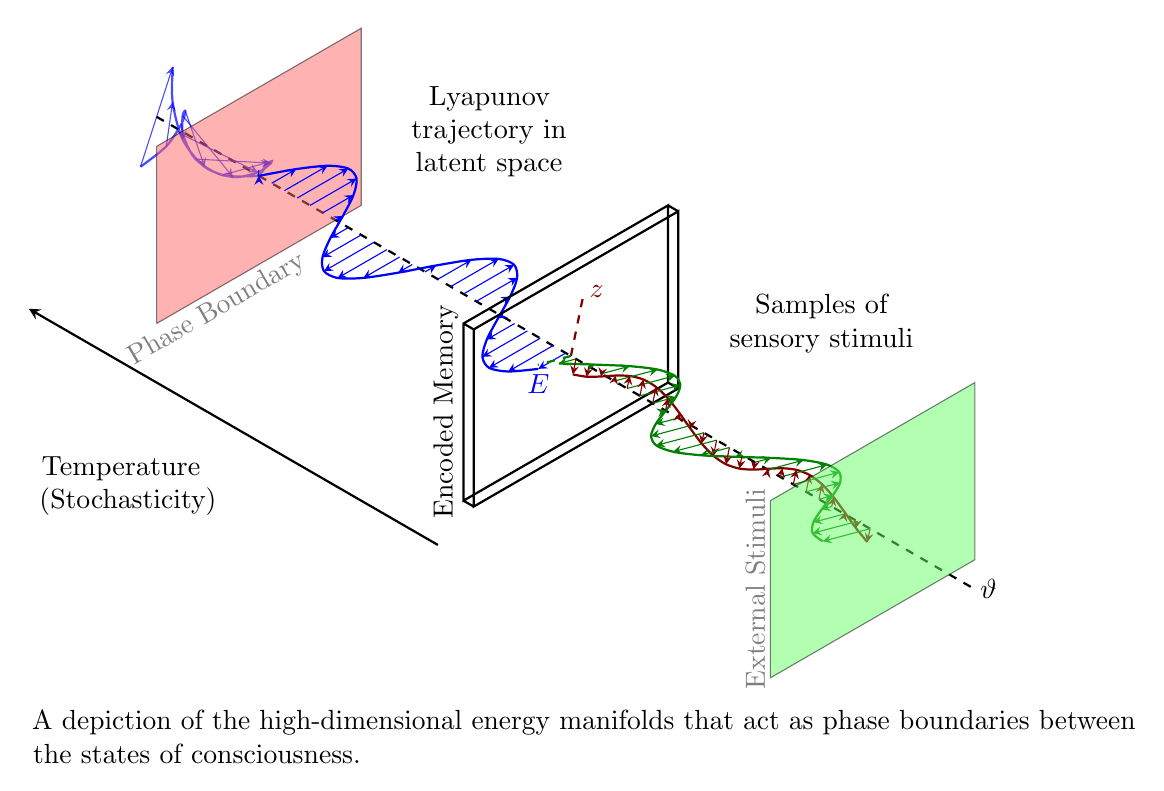
\begin{tikzpicture}[x={(0.866cm,-0.5cm)}, y={(0.866cm,0.5cm)}, z={(0cm,1cm)}, scale=.75,
    %Option for nice arrows
    >=stealth, %
    inner sep=0pt, outer sep=2pt,%
    axis/.style={thick,->},
    left_axis/.style={thick,<-},
    axis_2/.style={thick,-, opacity=1},
    wave/.style={thick,color=#1,smooth},
    polaroid/.style={fill=green!60!white, opacity=0.5},
    phase/.style={fill=red!60!white, opacity=0.5},
]
    % Colors
    \colorlet{darkgreen}{green!50!black}
    \colorlet{lightgreen}{green!80!black}
    \colorlet{darkred}{red!50!black}
    \colorlet{lightred}{red!80!black}

    % Frame
    \coordinate (O) at (0, 0, 0);
    \draw[axis_2, dashed] (O) -- +(14, 0,   0) node [right] {$\vartheta$};
    \draw[left_axis] (0, -4.5, 0) -- +(8, 0,0) node [left, text width=3cm](B) at (5.5, -5, 0) {Temperature  (Stochasticity)}; 
    % \draw[axis] (O) -- +(0,  2.5, 0) node [right] {z'};
    % \draw[axis] (O) -- +(0,  0,   2) node [above] {z};

    \draw[thick,dashed] (-2,0,0) -- (O);

    % monochromatic incident light with electric field
    \draw[wave=blue, opacity=0.7, variable=\x, samples at={-2,-1.75,...,0}]
        plot (\x, { cos(1.0*\x r)*sin(2.0*\x r)}, { sin(1.0*\x r)*sin(2.0*\x r)})
        plot (\x, {-cos(1.0*\x r)*sin(2.0*\x r)}, {-sin(1.0*\x r)*sin(2.0*\x r)});

    \foreach \x in{-2,-1.75,...,0}{
        \draw[color=blue, opacity=0.7,->]
            (\x,0,0) -- (\x, { cos(1.0*\x r)*sin(2.0*\x r)}, { sin(1.0*\x r)*sin(2.0*\x r)})
            (\x,0,0) -- (\x, {-cos(1.0*\x r)*sin(2.0*\x r)}, {-sin(1.0*\x r)*sin(2.0*\x r)});
    }

    \filldraw[phase] (0,-2,-1.5) -- (0,-2,1.5) -- (0,2,1.5) -- (0,2,-1.5) -- (0,-2,-1.5)
        node[below, sloped, near end]{Phase Boundary};%
        

    %Direction of polarization
    % \draw[thick,<->] (0,-1.75,-1) -- (0,-0.75,-1);

    % Electric field vectors
    \draw[wave=blue, variable=\x,samples at={0,0.25,...,6}]
        plot (\x,{sin(2*\x r)},0)node[anchor=north]{$E$};

    %Polarized light between polaroid and thin section
    \foreach \x in{0, 0.25,...,6}
        \draw[color=blue,->] (\x,0,0) -- (\x,{sin(2*\x r)},0);

    \draw (3,1.5,1.5) node [text width=2.5cm, text centered]{Lyapunov trajectory in latent space};

    %Crystal thin section
    \begin{scope}[thick]
        \draw (6,-2,-1.5) -- (6,-2,1.5) node [above, sloped, midway]{Encoded Memory}
                -- (6, 2, 1.5) -- (6, 2, -1.5) -- cycle % First face
            (6,  -2, -1.5) -- (6.2, -2,-1.5)
            (6,   2, -1.5) -- (6.2,  2,-1.5)
            (6,  -2,  1.5) -- (6.2, -2, 1.5)
            (6,   2,  1.5) -- (6.2,  2, 1.5)
            (6.2,-2, -1.5) -- (6.2, -2, 1.5) -- (6.2, 2, 1.5) 
                -- (6.2, 2, -1.5) -- cycle; % Second face

        %Optical indices
        \draw[darkred, dashed]       (6.1, 0, 0) -- (6.1, 0.26,  0.966) node [right] {$z$}; % index 1
        % \draw[darkred, dashed]   (6.1, 0, 0) -- (6.1,-0.26, -0.966) node [left] {$z$}; % index 1
        % \draw[darkgreen, ->]     (6.1, 0, 0) -- (6.1, 0.644,-0.173) node [right] {$n_{p}'$}; % index 2
        \draw[darkgreen, dashed] (6.1, 0, 0) -- (6.1,-0.644, 0.173); % index 2
    \end{scope}

    %Rays leaving thin section
    \draw[wave=darkred,   variable=\x, samples at={6.2,6.45,...,12}] 
        plot (\x, {0.26*0.26*sin(2*(\x-0.5) r)},  {0.966*0.26*sin(2*(\x-0.5) r)});  %n'g-oriented ray
    \draw[wave=darkgreen, variable=\x, samples at={6.2,6.45,...,12}]
        plot (\x, {0.966*0.966*sin(2*(\x-0.1) r)},{-0.26*0.966*sin(2*(\x-0.1) r)}); %n'p-oriented ray
    \draw (9.5,1.5,1.5) node [text width=2.5cm, text centered] {Samples of sensory stimuli};

    \foreach \x in{6.2,6.45,...,12} {
        \draw[color=darkgreen, ->] (\x, 0, 0) --
            (\x, {0.966*0.966*sin(2*(\x-0.1) r)}, {-0.26*0.966*sin(2*(\x-0.1) r)});
        \draw[color=darkred,   ->] (\x, 0, 0) --
            (\x, {0.26*0.26*sin(2*(\x-0.5) r)}, {0.966*0.26*sin(2*(\x-0.5) r)});
    }

    %Second polarization
    \draw[polaroid]   (12, -2,  -1.5) -- (12, -2,   1.5)  %Polarizing filter
        % 
        % below, sloped, near end
        node [above, sloped, midway] {External Stimuli} -- (12, 2, 1.5) -- (12, 2, -1.5) -- cycle;
    
    
    % \draw[thick, <->] (12, -1.5,-0.5) -- (12, -1.5, 0.5); %Polarization direction

    %Light leaving the second polaroid
    % \draw[wave=lightgreen,variable=\x, samples at={12, 12.25,..., 14}]
    %     plot (\x,{0}, {0.966*0.966*0.26*sin(2*(\x-0.5) r)}); %n'g polarized ray
    % \draw[wave=lightred,  variable=\x, samples at={12, 12.25,..., 14}]
    %     plot (\x,{0}, {-0.26*0.966*sin(2*(\x-0.1) r)});      %n'p polarized ray

    \node[align=justify, text width=14cm, anchor=north west, yshift=-2mm] at (current bounding box.south west)
        {A depiction of the high-dimensional energy manifolds that act as phase boundaries between the states of consciousness. };
\end{tikzpicture}
% The third axis indicates an increasing stochasticity in the environment which results from information loss being supplemented by generated synthetic data.
\end{center}

\newpage

\section{Overview}

Energy-based models (EBMs) provide an alternative perspective to the standard optimization approach of using a cost function to measure a model's ability to learn a probability density. This provides a useful layer of abstraction to build on and may also be more computationally efficient by avoiding computing an intractable posterior and only computing variable dependencies. A phase space that is divided by two manifolds described by separate energy functions that represent phase boundaries of the three states in which the agent can exist is proposed. The approach of maintaining two energy functions is in contrast to the standard approach of minimizing a single cost function. Having a mixture between an true world model and an upper bound of incoherent reality allows for better predictions within a stochastic test environment and also encourages creative experimentation and imaginative exploration. 

%% Description of the agent and and its dynamic movement, some mention of stochasticity in environment
In thermodynamics, a dissipative system is an open system that exchanges energy with an environment. One notion of a dissipative system is the existence of a Lyapunov function. By dynamically optimizing the internal parameters of an agent we can minimize the free energy represented by a Lyapunov function that contains a Kullback–Leibler divergence or relative entropy of the joint energies. At higher states, the temperature or stochastic nature of the environment grows, which decreases the stability of the dissapative agent and increases the likelihood that it crosses a phase boundary and transitions its state. The degree of randomness in the environment corresponds to information loss that results from repeatedly encoding latent observations. 

%% Description of The environment
If we label the three states an agent can exist in as \textit{waking} consciousness, \textit{dreaming} consciousness, and \textit{lucid dreaming} consciousness we establish a model of the mind. The lowest phase space is observable reality and the phase space between the two manifolds is the dream world. It is sufficiently distanced so that prediction errors, which can be interpreted as confabulation, do not necessarily push the agent into a phase transition. The lower phase boundary, dividing waking and dreaming consciousness, is the encoded discriminator's energy function, $E_{\text{world}}$. This can be interpreted as a collection of observations of reality from the training data and any highly plausible generated predictions. This manifold serves as the lower bound or ground truth of the agent's world model. The higher phase boundary, dividing dreaming and lucid dreaming consciousness, is the energy manifold of a highly stochastic generative model, $E_{\text{dream}}$.  After passing the phase boundary into dream lucidity,  information sampled by the agent is interpreted with access to both discriminators. In such a state, an agent is aware of both the dream world implausibility and the constraints of reality. From this vantage point, a system can temporarily distill knowledge and explore abstractions of a highly stochastic reality. By considering this metaphysical structure  as a model of our consciousness, we open two paths of exploration in dream research and as an approach to developing human-like creative exploration in artificial agents.

% Lucid dreaming consciousness can be interpreted as a form of secondary consciousness that performs knowledge distillation of the ensemble density of the dream world and the memory of experienced reality. 
% When we dream, we enter the phase space between the accurate world model and a world model of minimal plausibility. Here, the parameters of our internal states are in continuous flux in order to resist phase transitions into waking or lucid dreaming states.
% After passing the phase boundary into lucidity, latent space can be interpreted as a closed loop with information being interpreted as external stimuli.


\section{Training the Energy Functions}

% https://colab.research.google.com/drive/1zNR0KbIz9RsJxJ5DBXrTOM2JSFLDQMCy


In a standard training algorithm, we aim to minimize a loss from a cost function. In terms of our energy-based model, this would be equivalent to minimizing the space between the generative world model to make it as close to the training data as possible. This results in an artificial intelligence agent that exists as closely in the waking state as possible but lacks imaginative abilities. Instead, we train an artificial agent to have both a realistic model of the world but also be able to have an understanding of how to creatively modify its world model to some extreme. Moreover, the agent should be able to validate these modifications, store its ideas in memory, and later decode and re-enact the useful ideas on the external world environment. 
\begin{figure}[H]
    \centering
    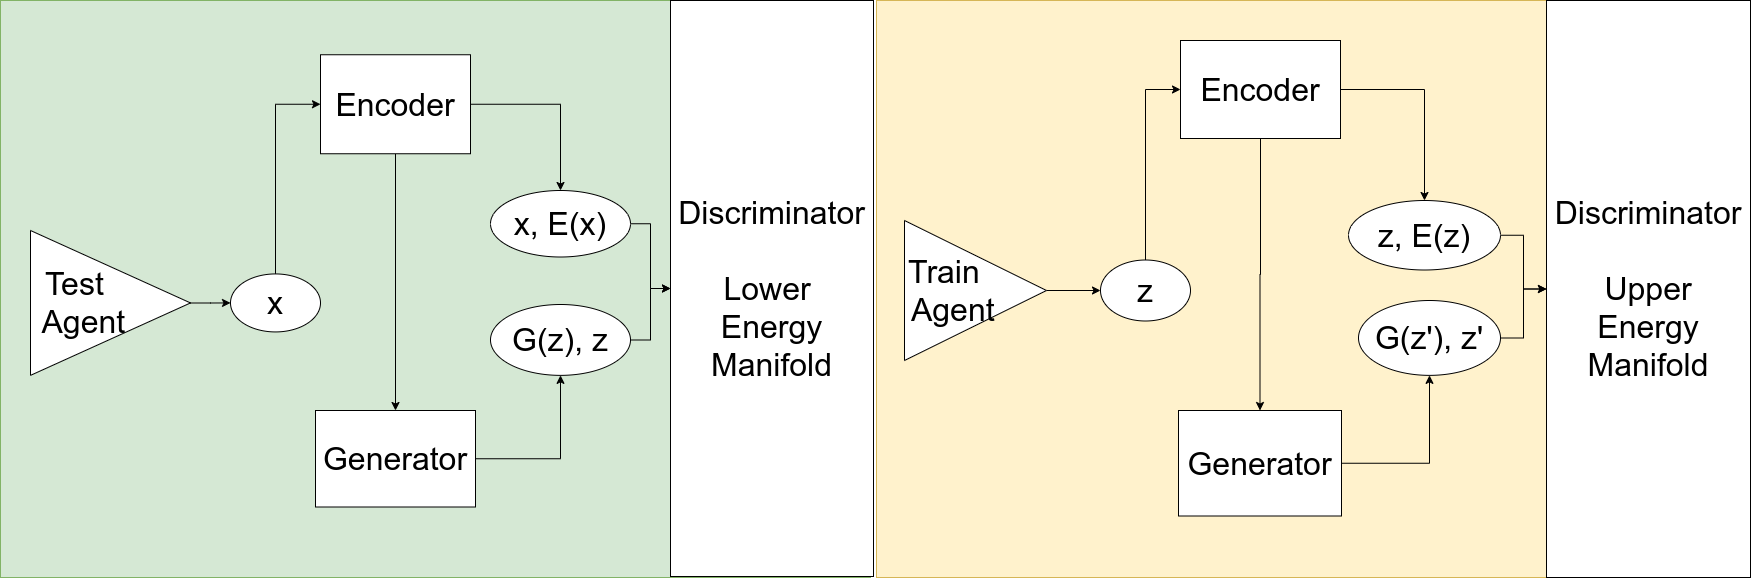
\includegraphics[width=13.9cm]{dream-model-v2.png}
    % 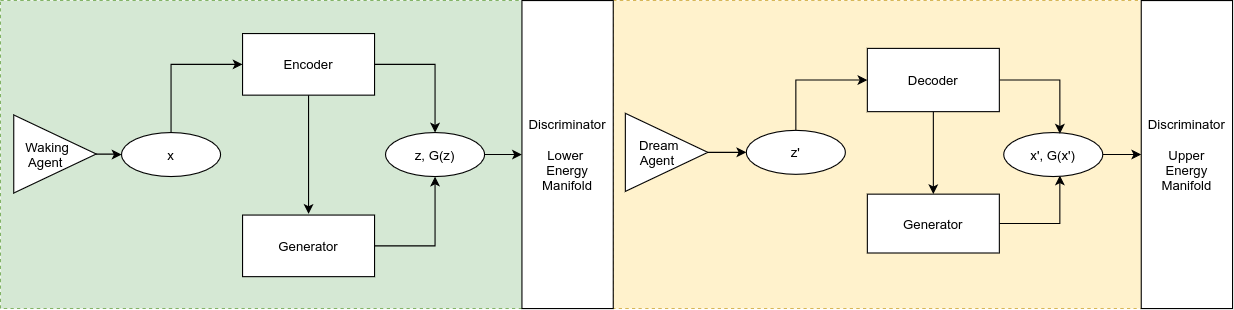
\includegraphics[width=13.9cm, height=4.5cm]{wake-dream-model.png}
    % \caption{Caption}
    % \label{fig:my_label}
\end{figure}

There are two phases of training, waking and dreaming, which occur sequentially. In the waking phase, an agent explores the external environment and creates an accurate model of the world. It does this by first encoding its sensory data, then producing synthetic predictions using the latent representation and training a discriminator on the tuple of outputs. This discriminator will be the lower energy manifold that acts as a phase boundary between the waking and dreaming state.  In the dreaming phase, the agent no longer has access to external sensory stimuli so it explores a latent environment. It performs a secondary encoding of its latent states, then generates synthetic predictions and trains a discriminator on the tuple of outputs. The dream model is able to produce highly implausible and incoherent data up to some coherency threshold. This threshold can be seen to be proportional to the dimensional difference between the information bottleneck of the encoder and the original dimension of the input. The energy function of this secondary discriminator will serve as the upper manifold, beyond which the environment becomes incoherent.

Both phases use a Bidirectional Generative Adversarial Networks (BiGAN) (Donahue et al. 2017) architecture. In addition to a generator $G$ from the standard GAN framework (Goodfellow et al., 2014), a BiGAN includes an encoder $E$ which maps input $x$ to its latent representations $z$. The BiGAN discriminator $D$  will jointly discriminate in both data space and latent space using tuples ($x$, $E(x)$) versus ($G(z)$, $z$). It can be proven that the BiGAN's encoder and generator must learn to invert one another in order to fool the BiGAN discriminator in an adversarial game. The process is repeated in latent space during dreaming phase with latent data being further distilled. By reusing the encoder and generator in both phases, we are able to have encoding and generative mechanisms that perform well at both levels of abstractions. 


% In a sense, this approach is similar to the World Models architecture (Ha and Schmidhuber, 2020). However, instead of using a Mixture Density Network combined with a RNN (MDN-RNN) to predict a range of stochastic states, the trajectories of a dynamical system will be computed by minimizing free energy of a composition of these bounding densities in order to train the actions and sampling of the agent. 

\section{The Free Energy Principle}

% Biological systems are thermodynamically open, in that they exchange energy and entropy with their environment. They operate far-from-equilibrium and are dissipative, showing self-organizing behaviour. However, they can negotiate a changing or non-stationary environment in a way that allows them to endure over substantial periods of time. This endurance means that they avoid phase transitions that would otherwise change their physical structure .
The free energy principle can be used to describe how thermodynamically open biological systems negotiate a changing or non-stationary environment in a way that allows them to endure over substantial periods of time (Friston, 2006). Let $\vartheta$ parameterize environmental forces or fields that act upon the agent and $\lambda$ be quantities or temperature that describe the agents physical state. The free energy is a scalar function of the ensemble density and the current sensory input. Let $q(\vartheta ;\lambda)$ be an arbitrary density function on the environments parameters that is specified or encoded by the agents parameters. It can be regarded as the probability density that a specific environmental state $\vartheta$ would be selected from an infinite ensemble of environments given the agents state $\lambda$, which is fixed and known. Then the free energy of the agent is given by, 
\begin{align}\label{eq:free-energy-1}
\begin{split} 
    F &= \int q(\vartheta) \ln \frac{p(\Tilde{y},\vartheta)}{q(\vartheta)} d\vartheta \\
    &= - \langle \ln p(\Tilde{y},\vartheta) \rangle_q + \langle \ln q(\vartheta) \rangle_q
\end{split}
\end{align}
Here $\langle \cdot \rangle_q$ means the expectation under the ensemble density $q$.

% Include diagram of phase space.

% Define variables and give formal description.

% \section{Network Architectures}



\section{Training and Testing the Agent}

A Lyapunov function is constructed to represent the composition of the two energy functions. A Lyapunov function is a scalar function of a systems state that decreases with time. Instead of trying to infer the Lyapunov function given an agent's structure and behaviour, we train the agent to minimize its Lyapunov function (its free energy) by optimizing its parameters. The free energy principle states that all the quantities that that are owned by the system will change to minimize free energy. These quantities are the agent's internal parameters $\lambda$ and the action parameters $\alpha$. We can rearrange $\eqref{eq:free-energy-1}$ to show the dependence of the free energy on $\alpha$ and $\lambda$,
\begin{align}\label{eq:free-energy-2}
\begin{split}
F &= -\ln p (\Tilde{y}) + D(q(\vartheta;\lambda) || p(\vartheta|\Tilde{y}))\\
&=  - \langle \ln p(\Tilde{y},\vartheta) \rangle_q + D(q(\vartheta;\lambda) || p(\vartheta|\Tilde{y}))
\end{split}
\end{align}

Where $D$ is the Kullback–Leibler cross-entropy or divergence term that measures the difference between the ensemble density and the conditional density of the causes. Changing the configuration of the system to move or resample the environment by optimizing its actions $\alpha$ will minimize the free energy of the first term. The Kullback–Leibler divergence $D$ is used to descend the Lyapunov free energy by optimizing the agents internal parameters $\lambda$ in the second term with,
\[
D(q(\vartheta;\lambda) = \int q \ln \frac{q}{p} d\vartheta.
\]
By minimizing its free energy, the agent learns how to act in order for its trajectories to stabilize by descending into basins of attractions to find equilibrium points. It follows that the latent trajectories can be interpreted with symbolic dynamics. A symbolic orbit is a sequence of symbols corresponding to the successive partition elements visited by the point in its orbit. Instead, we use an Autoencoder to learn an encoding that will partition the space, which reduces the memory and computation of what would otherwise involve solving high dimensional differential equations on a continuous domain.

% During the waking phasing, the agent now has access to both the discriminators and generators of the world model and the upper bounded dream model. It can simultaneously use them to predict and imagine in order to make the best decisions over a wider range of possible states.


% What are the equilibrium points? Goals or objectives?

% \section{Hopfield Closed-Loop}

% An interesting idea is to use a Hopfield Network to encode sequential memory patterns into an energy manifold during wake phase training. When sleeping we can consider the phase space as a closed loop.

% From here, we attent to minimize the energy

% \section{Knowledge Distillation of Multi-Agents}

% TODO: Read why computing trajectory is computationally infeasible. Consider multi-agent persona sampling: each persona has a tendency to behave differently (more aggressive, passive, etc.) the model samples from multi-agents and selects actions that minimize energy in environment.

% The space of dreams may be vast and largely not very useful. Hinton makes an interesting analogy between an ensemble of multiple neural networks being trained on specific features with the composition of matter in the universe. He shows that a large portion of the information being stored in the ensemble of networks is actually redundant and is a kind of dark knowledge. In order to minimize the amount of computation and the model's memory footprint, this dark knowledge can distilled by training a new model using a softmax or logits of all the models. These operations reduce the range of information stored in the outputs while maintaining accuracy of relative dependencies in the distilled model.

% It is conceivable that a similar process occurs in our minds during dreaming sleep where the single agent we understand as our base consciousness self-replicates its core parameters into a multi-agent representation with a further distilled set of features. Instead of casting out single fishing rods to search the phase space, we can cast out an entire net. This allows us to simulate multiple latent trajectories and better explore the phase space in search of equilibrium points of interest. Since computations using lower-dimensional latent representations are less expensive, it is conceivable for the mind to be able to run multiple latent trajectories in parallel. That is, our base consciousness periodically switches between its replicated agents by selecting agents with Lyapunov trajectories that have minimal positive energies with $E>0$ and are strictly decreasing  with $\frac{dE}{dt} < 0$. This enables the selection of agents that are nearest to approaching an equilibrium point using a variation of initial conditions in the environment. These points are of interest because they capture highly stochastic yet highly plausible states of the world model that haven't yet been experienced. 

% The base model then decodes the current best trajectory from its latent representation into a sensory representation until it converges or a periodic transition occurs to the next best if the trajectory becomes stale.A fter discovering equilibrium points, the manifolds are updated to capture the stability point where the two boundaries intersect.

% They represent semantic areas that ascend into dream lucidity but still maintain a minimal amount of  realistic stochasticity and thus remain coherent.

% Describe dark knowledge of dream world.

% Describe knowledge distillation of ensemble density of dream and reality.

% Analyze usefulness of pushing agent past upper phase transition into highly stochastic environment.

\section{Discussion}

% Work In Progress 

It is conceivable that the state of a dreaming artificial intelligence agent can be pushed to transition phases into lucidity, which is a higher analog of the shallow consciousness experienced when being trained solely on sensory inputs. It's unknown what role dream lucidity plays in the development of consciousness or creativity. In a simulation game, we may attempt to use lucidity of a computer to unveil tactics or strategies that we were unaware of in order to improve our performance and our understanding of the game. 
% It can be posited that the game of consciousness is the interplay between man and machine within nested simulation.

It is also conceivable that the dissapative state of lucid dreaming in humans can be extended using an external system to provide perturbations that drive a dreaming consciousness to transition phases into lucid dreaming consciousness and stabilize in this state. In this state we would be able to freely modify our world without being constrained by physical reality or our physical abilities. From here, it may be possible to store and later decode our imagined actions and ideas from dreams to reality. 


% Likewise, a machine may be using us to unveil tactics in a simulation. Creation of a simulation could be evidence of our own existence in a simulation. 

% \section{Appendix}

% \subsection{Energy-Based Models}
% \textit{See EBM course notes by Yann Lecun:}
% \begin{center}
% \url{https://atcold.github.io/pytorch-Deep-Learning/en/week07/07-1/}
% \end{center}

% \subsection{Dream Research}

% Dreams can be described as sensorimotor hallucinatory experiences that follow a narrative structure (Nir and Tononi, 2010). There is some evidence that dreams, like output from generators, are also created in a top-down manner. That is, they originate in abstract knowledge and figurative thought and are then processed back into imaginal copies of perceptual phenomena. Dream recall was found to correlate best with abilities of mental imagery rather than language proficiency.

% Children under the age of 7 reported dreaming only 20\% of the time when awakened from REM sleep, compared with 80–90\% in adults. Visuo-spatial skills are known to depend on the parietal lobes, which are not fully myelinated until age 7. Lesion studies also find a cessation of dreaming follows from damage in or near the temporo-parieto-occipital junction. Some lesions are associated with increased frequency and vividness of dreams and their intrusion into waking life, especially those in medial prefrontal cortex, the anterior cingulate cortex, and the basal forebrain.

% In the Block Design Test of the Wechsler intelligence test battery, children look at models or pictures of red and white patterns, and then recreate those patterns with blocks. Scores on this test are the one parameter that correlates best with dream report in children. Children with the most developed mental imagery and visuo-spatial skills (rather than verbal or memory capabilities) report the most dreams.

% In the mental rotation test, a subject is asked to determine whether two figures are the same or different given images of their rotated states. To perform well in this test, the subject needs to have a well-developed and functioning visuo-spatial and mental imagery skills since the act of rotating the object is a form of imagining.

% An Autoencoder is trained to encode sensory input into latent variables

% Overparameterized autoencoders can be trained to implement associative memory via iterative maps
% https://arxiv.org/pdf/2006.16540.pdf

% Hopfield layer can be used as a plug-in replacement for permutation equivariant layers. Since the Hopfield layer is an associative memory it assumes no dependency between the input patterns.

% Hopfield layer can act as an attention layer, where state (query) and stored (key) patterns are different, and need to be associated.

% Hopfield layer can be used as a plug-in replacement for GRU \& LSTM layers. Optionally, for substituting GRU \& LSTM layers, positional encoding might be considered.

\section*{References}

\small

[1] Friston, K.J., Stephan, K.E. Free-energy and the brain. Synthese 159, 417–458 (2007). 

[2] J. Donahue, P. Krahenbuhl, and T. Darrell. Adversarial feature learning. arXiv preprint arXiv:1605.09782, 2016.

% [2] D. Ha and J. Schmidhuber. World models. In Advances in Neural Information Processing Systems (NIPS), 2018.

% [3] Friston KJ, Daunizeau J, Kiebel SJ (2009) Reinforcement Learning or Active Inference?. PLoS ONE 4(7): e6421. doi:10.1371/journal.pone.0006421

% [4] G. Hinton, O. Vinyals, and J. Dean. Distilling the knowledge in a neural network. arXiv preprint arXiv:1503.02531, 2015.

[3] Ian Goodfellow, Jean Pouget-Abadie, Mehdi Mirza, Bing Xu, David Warde-Farley, Sherjil Ozair, Aaron Courville, and Yoshua Bengio. Generative adversarial nets. In NIPS, 2014.

% [4] Hafner D, Ortega P, Ba J, Parr T, Friston K.J, Heess N. Action and Perception as Divergence Minimization. (2020). 

[4] Nir Y, Tononi G. Dreaming and the brain: from phenomenology to neurophysiology. Trends Cogn Sci. 2010;14(2):88-100. doi:10.1016/j.tics.2009.12.001



\vspace{2cm}

% \author{%
%   Luke J. Pereira \\
%   \texttt{lukejoepereira@gmail.com} \\
% }

% \begin{displayquote}
% You cannot swim for new horizons until you have courage to lose sight of the shore
% \textbf{--- William Faulkner}
% \end{displayquote}

\end{document}
